% Chapter Template

\chapter{SCgPC and HDMR for Fuel Pin Cell} % Main chapter title

\label{ch:mammoth} % Change X to a consecutive number; for referencing this chapter elsewhere, use \ref{ChapterX}

\lhead{Chapter 8. \emph{Fuel Pin Cell}} % Change X to a consecutive number; this is for the header on each page - perhaps a shortened title

%----------------------------------------------------------------------------------------
%	SECTION: INTRO
%----------------------------------------------------------------------------------------

\section{Introduction}
While analytic models provide insight to the operation of stochastic collocation for generalized polynomial chaos and high-density
model reduction methods, we are chiefly interested in applying these methods to engineering applications that lead to
decision making in real-world activities.  
In Chapter \ref{ch:c5g7}, we demonstrated SCgPC and HDMR methods on a single-physics neutron transport model
with several responses.  We turn attention now to a more complicated multiphysics model whose physics are not
simple to describe in their entirety.
To this end, we selected a model solved by multiphysics simulation code \mammoth{}, a \moose{}-based
code that couples neutronics code \rattlesnake{} \cite{rattlesnake} and fuel performance code \bison{}
\cite{bison}.

We discussed the neutronics solved by \rattlesnake{} in Chapter \ref{ch:c5g7}.  For this particular
application, we will not make the diffusion approximation, but track neutrons in discrete angles of travel
in the neutron transport equation instead \cite{lewistrans}.  \bison{} solves several physical models as part
of fuels performance.  As described in the code documentation, for light-water nuclear reactors \bison{} models 
fuel oxidation behavior through
temperature, burnup, and porosity-dependent material properties, volumetric heat generation, thermal fission
product swelling and densification, thermal and irradiation creep, fuel fracture via relocation, and fission
gas release.  In addition, it models heat transfer through interstitial gaps in the fuel-cladding
construction, mechanical contact, plenum pressure, cladding creep and thermal expansion, cladding plasticity,
and coolant heat transfer coefficients.  There are equations for each of these phenomena that are too
extensive to cover in this work; we refer instead to the \bison{} documentation \cite{bison}.

The coupling between \rattlesnake{} and \bison{} is two-way and involves an iterative process.  The neutronics
solved in \rattlesnake{} determines the shape of the distribution of neutrons in the domain, often referred to
as the \emph{power shape}.  The fuels performance code uses this power shape to determine temperatures
throughout the domain and determine all of the resulting changes in performance because of the physics
mentioned above.  The temperature calculated is then provided as feedback to neutronics, which adjusts the
material cross sections accordingly.  These two physics iterate using Picard iterations until they reach a
specified maximum number of iterations or converge to a specified tolerance.

\section{Problem}

The specific model to simulate is a coupled multiphysics engineering-scale model documented in \cite{physormammoth}.  
It simulates fuel behavior for a pressurized
water reactor fuel rod as it is used as fuel in a nuclear reactor.  It simulates fuel behavior through the 
depletion of fissile material over a year-long process without reactor power changes.
The domain is a single two-dimensional slice of a fuel rod.  The mesh contains fuel, gap, clad, and
moderator, and represents a symmetric quarter pin cell.  
The response of interest is the $k$-eigenvalue of the infinite reactor.

There are two meshes used in this coupled model, one each for \bison{} and \rattlesnake{}.  The distinction is
necessary because of the physics solved by each.  In \bison{} it is important to not mesh the gap between fuel
and cladding, as in the limit that the fuel expands and makes contact with the cladding, the gap mesh cells
will become infinitely long and thin.  This causes a number of numerical errors.  For \rattlesnake{} however
it is critical to mesh the gap, as neutron transport will be affected by the materials of the gap.  The two
meshes are shown in Figures \ref{fig:pincell fuel mesh} and \ref{fig:pincell neutron mesh}.
The meshes each contain 20 rings of fuel element groups (red) and the clad (green),
and the neutronics mesh additionally contains the gap (yellow) and the moderator (blue).  
The fuel pin radius is 4.09575 millimeters including the cladding, and the domain including the moderator is
from 0 to 6.3 millimeters square.  The boundaries are reflective on all sides to simulate operation in an
infinite reactor.

\begin{figure}[H]
  \centering
  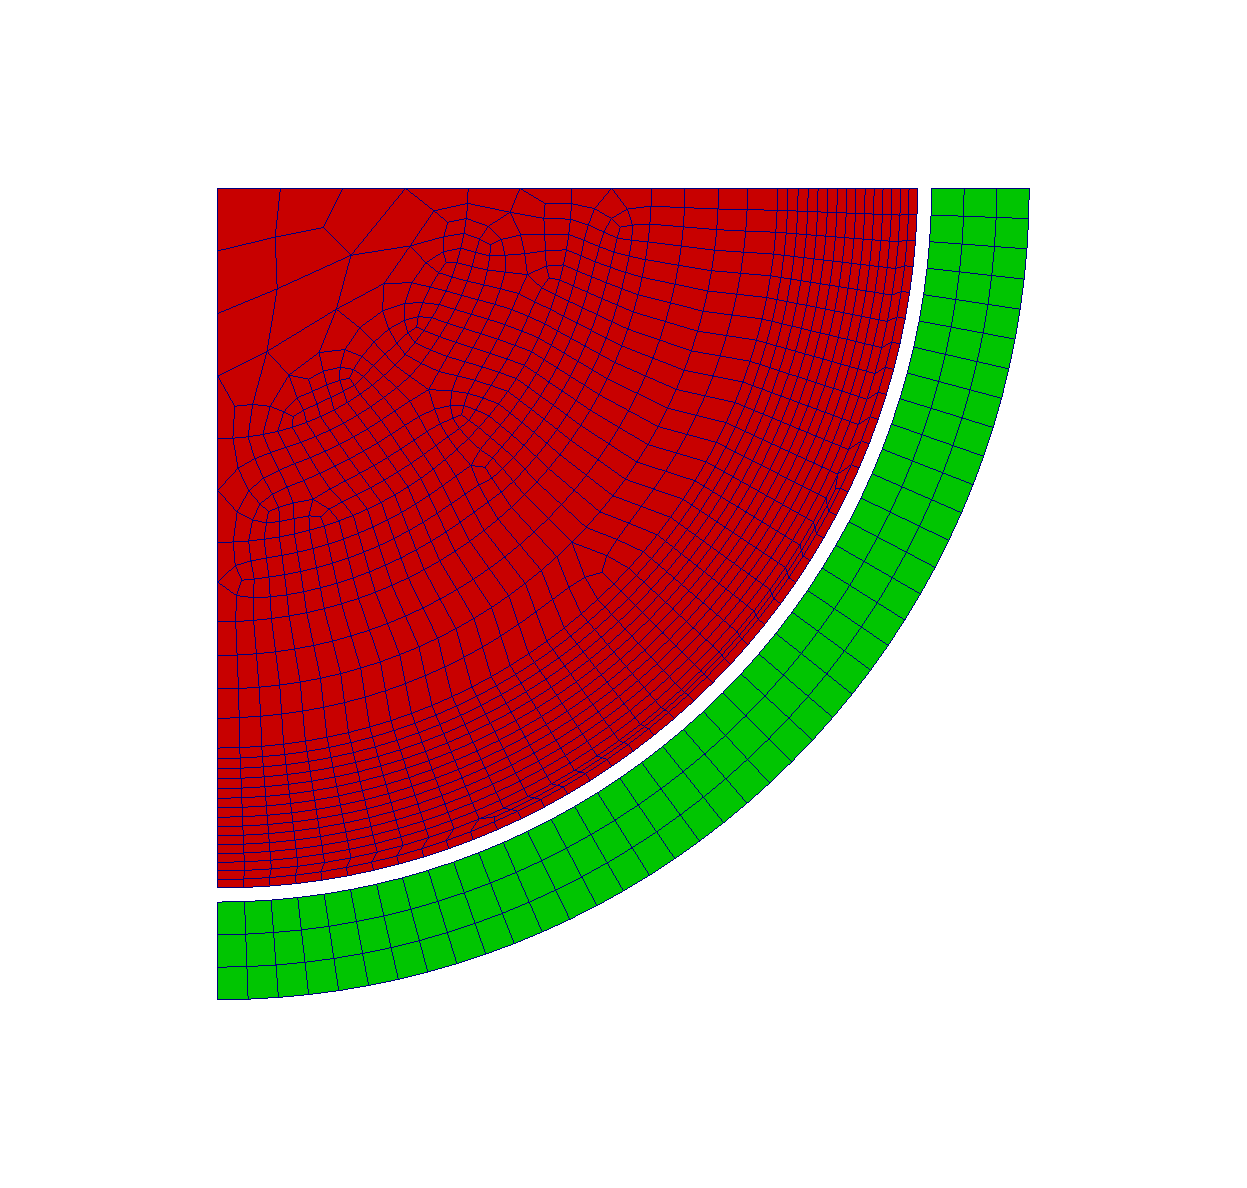
\includegraphics[width=0.7\linewidth]{mammoth/FuelsMesh}
  \caption{Pincell Mesh for Fuels Performance \cite{physormammoth}}
  \label{fig:pincell fuel mesh}
\end{figure}
\begin{figure}[H]
  \centering
  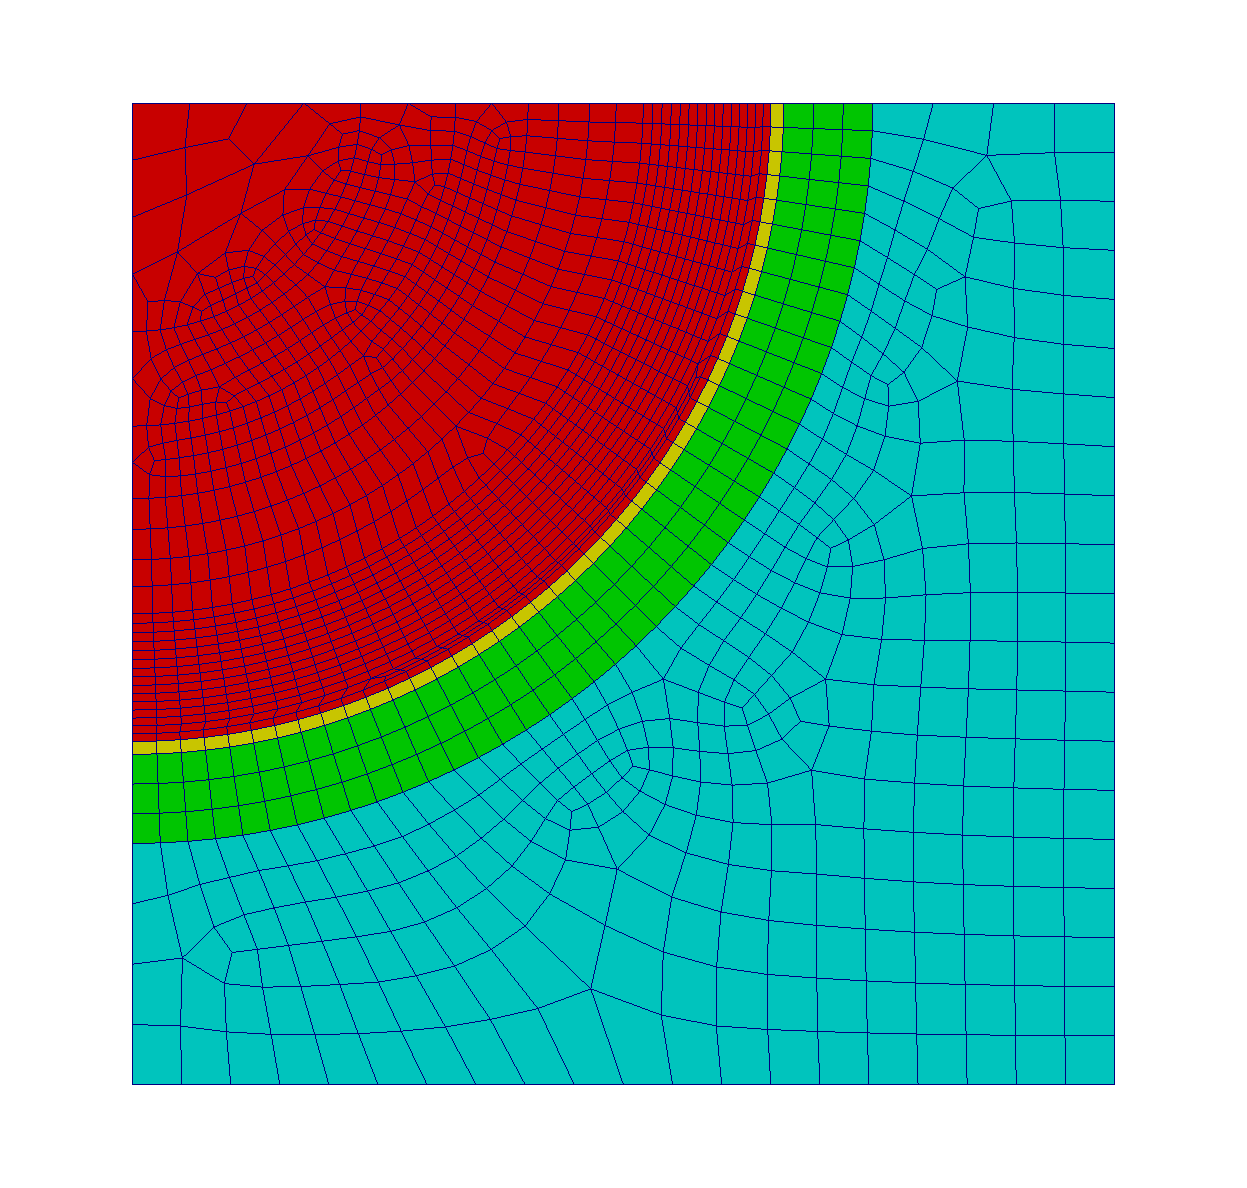
\includegraphics[width=0.7\linewidth]{mammoth/NeutronicsMesh}
  \caption{Pincell Mesh for Neutronics \cite{physormammoth}}
  \label{fig:pincell neutron mesh}
\end{figure}

The neutronics is calculated using 8 energy groups and second-order level-symmetric quadrature for angle, and 
takes as uncertain inputs 671 material cross
sections, including fission, capture, scattering, and neutron multiplication factor.  Variance and covariance
data was previously collected for these inputs using cross section code \texttt{SCALE} \cite{scale} with a Monte Carlo (MC)
random sampling approach.  In an effort to capture more interesting physics and uncertainties, the covariance
matrix was scaled up uniformly by a factor of 10 for this work.  The resulting covariance matrix was used to
construct a multidimensional Gaussian distribution.  Additionally, we perturb three material properties from
the \bison{} simulation: the fuel thermal expansion coefficient, fuel thermal conductivity, and cladding
thermal conductivity.  The uncertain distribution for these parameters are provided in Table 
\ref{tab:pincell bison distros}.  Note that the fuel thermal conductivity is in actuality a scaling factor to
the value used within \bison{}, which is calculated based on changing material properties.
\begin{table}
  \centering
  \begin{tabular}{c|c c|c}
    Parameter & Mean & Std. Dev. & Units \\ \hline
    Fuel Thermal Expansion Coefficient & $1\times10^{-5}$ & $7.5\times10^{-7}$ & /K\\
    Clad Thermal Conductivity & 16 & 2.5 & W/m-K\\
    Fuel Thermal Conductivity (Scale Factor) & 1 & 0.075 & --
  \end{tabular}
  \caption{\bison{} Uncertain Input Parameters}
  \label{tab:pincell bison distros}
\end{table}

The neutronics uncertain input space is highly correlated, so a Karhunen-Loeve (KL) component analysis and
associated sensitivity analysis is performed as
two-part reduction \cite{physor2016} in \raven{} similar to the process for the neutronics model
in Chapter \ref{ch:c5g7}.  The resulting variables and distributions are \emph{latent} inputs and can be
translated back to the \emph{manifest} (original) space by way of a transformation matrix.
Table \ref{tab:pcarank} gives the first several importance ranking eigenvalues for latent variables, which are
identified only by their ranking in the KL expansion.  We elected to truncate at 20 input variables.  
Figure \ref{fig:pincell impranks} shows the importance rank
information graphically.  The red cross line associated with the left y-axis shows the importance rank
eigenvalue for each latent variable, sorted by value.  The blue circle line associated with the right y-axis
shows the cumulative importance obtained by keeping any number of the latent inputs.  We note that in both
cases the x-axis is log scale; this is because the importance eigenvalues drop off quite quickly, and we wish
to emphasize the first eigenvalues over the remainder.  We also add a black line to the plot and chart
to indicate where the truncation was performed.

\begin{table}[H]
  \centering
  \begin{tabular}{c|c}
KL Rank & Importance Eigenvalue \\ \hline
0 & 0.385343134782 \\
2 & 0.178983653121 \\
8 & 0.136388464634 \\
7 & 0.0490658001469 \\
4 & 0.0259995867302 \\
12 & 0.0192003280782 \\
3 & 0.0159149198373 \\
18 & 0.0137261803754 \\
10 & 0.0119423872093 \\
14 & 0.0116995399806 \\
11 & 0.0105619452358 \\
1 & 0.00930331126013 \\
19 & 0.00772899277483 \\
6 & 0.00699483215964 \\
15 & 0.00682086107147 \\
28 & 0.00601178948093 \\
17 & 0.00515798964297 \\
16 & 0.00453075658143 \\
25 & 0.00402772081725 \\
9 & 0.00368309194804 \\ \hline
23 & 0.0029116602401 \\
21 & 0.00220070148712 \\
13 & 0.00219721801241 \\
5 & 0.00130555372756
\end{tabular}
\caption{KL Expansion Eigenvalues for Pin Cell Problem}
\label{tab:pcarank}
\end{table}

\begin{figure}
  \centering
  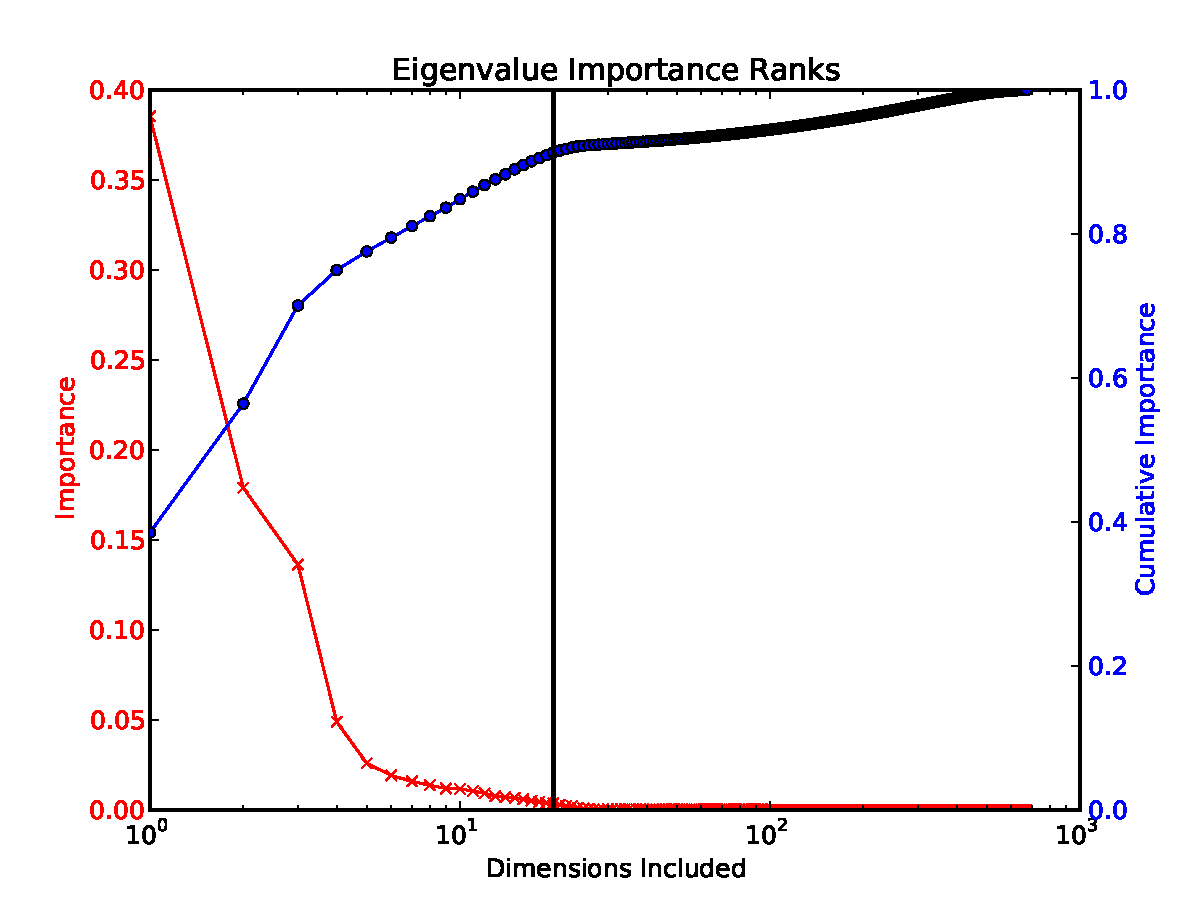
\includegraphics[width=0.7\linewidth]{mammoth/pincell_eigenvalue_impranks}
  \caption{Pincell $k$-Eigenvalue Importance Ranks}
  \label{fig:pincell impranks}
\end{figure}

\moose{} and its applications including \rattlesnake{}, \bison{}, and \mammoth{} do not generally have a
versioning system or release
schedule; instead, it is tracked by \texttt{Git} \cite{git} commit hashes.
This computation was performed with the application versions listed in Table \ref{tab:git}.  There is nothing
particularly special about these versions, except that they were concurrent and compatible at the time
calculations were performed.
\begin{table}
  \centering
  \begin{tabular}{c c}
    App & Git Version Hash \\ \hline
    \moose{ } & 1fea13a34357a56c6fd049a239e57d597b1c277e\\
    \bison{ } & 5552eca741fa30be0efdefd35fecd954b47c9586\\
    \rattlesnake{ } & 2c892fad29ed7d1f7fb9833116d2b718f7b72055\\
    \mammoth{ } & be676b5974f990a0d2a7589ab2a2e58163a47b22 \\ \hline
    \raven{ } & 8f7c477740a8277c536d9bd6734614615a8b5cb7
  \end{tabular}
  \caption{Application Versions Used}
  \label{tab:git}
\end{table}

\section{Limitations}
During the collection of data, it was discovered that the performance of \bison{} can fluctuate depending on
the way is is parallelized.  There were instances where \bison{} would fail to converge, but report an unconverged
temperature as a converged solution.  As a result, there is artifical numerical error that is difficult to track or
account for.  Regardless, we demonstrate the performance of various uncertainty quantification methods on this model, 
as this behavior indicates true simulation behavior.  This issue was submitted to the \bison{} and \mammoth{}
developers for consideration in the future.

\section{Results}
Figures \ref{fig:mammoth mean} and \ref{fig:mammoth var} show the values obtained for the mean and variance of
the $k$-effective response for a selection of uncertainty quantification methods, including
MC, static SCgPC using the total degree polynomial
construction indices, 
first- and second-order static HDMR,
and adaptive HDMR using both adaptive cut-HDMR and adaptive SCgPC.
 For additional clarity, we provide graphs centered more especially on the non-Monte
Carlo data in Figures \ref{fig:mammoth mean zoom} and \ref{fig:mammoth var zoom}.  Because the number of MC
samples necessary to obtain a well-resolved benchmark is prohibitive, we do not present any error
convergence plots for this model.

\begin{figure}[htb]
  \centering
  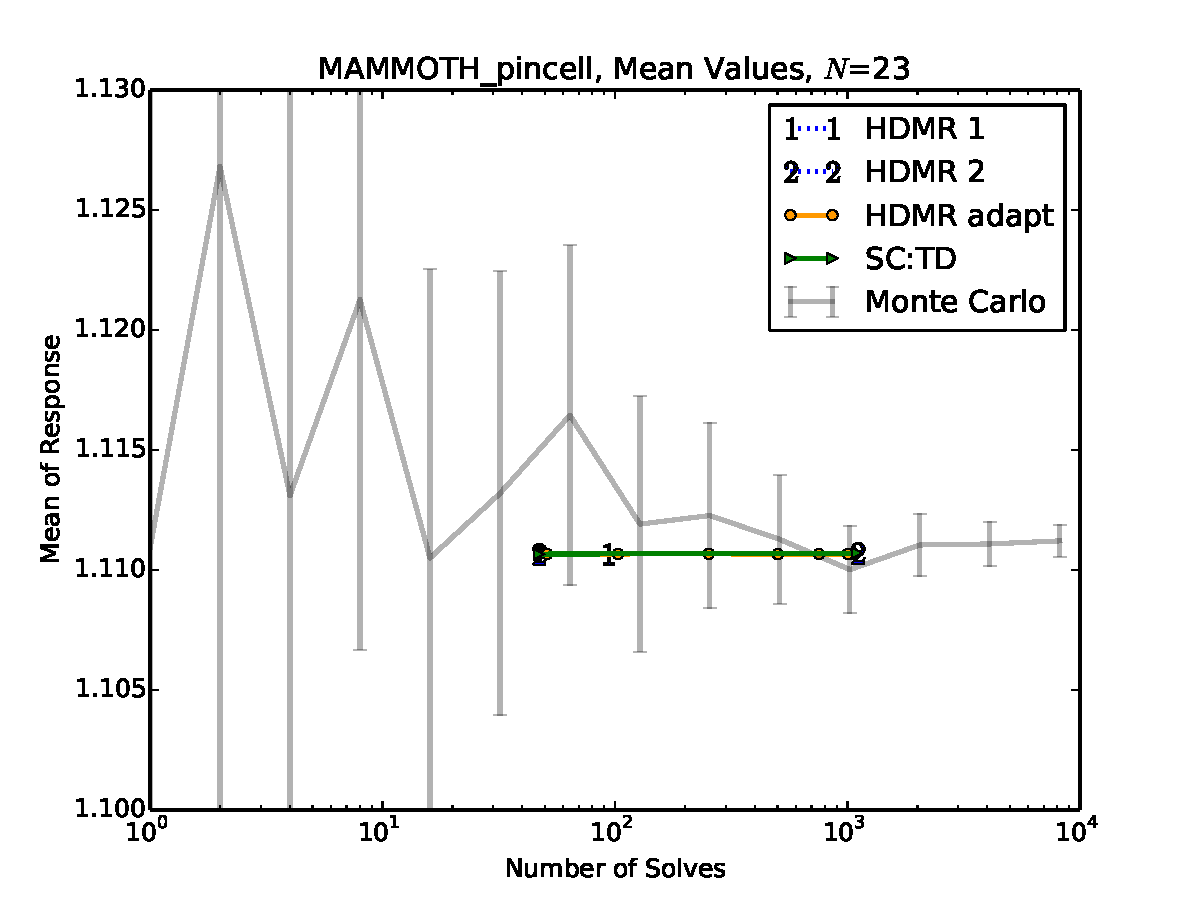
\includegraphics[width=0.7\linewidth]{mammoth/MAMMOTH_pincell_mean_vals}
  \caption{MAMMOTH Pin Cell, Mean Values}
  \label{fig:mammoth mean}
\end{figure}
\begin{figure}[htb]
  \centering
  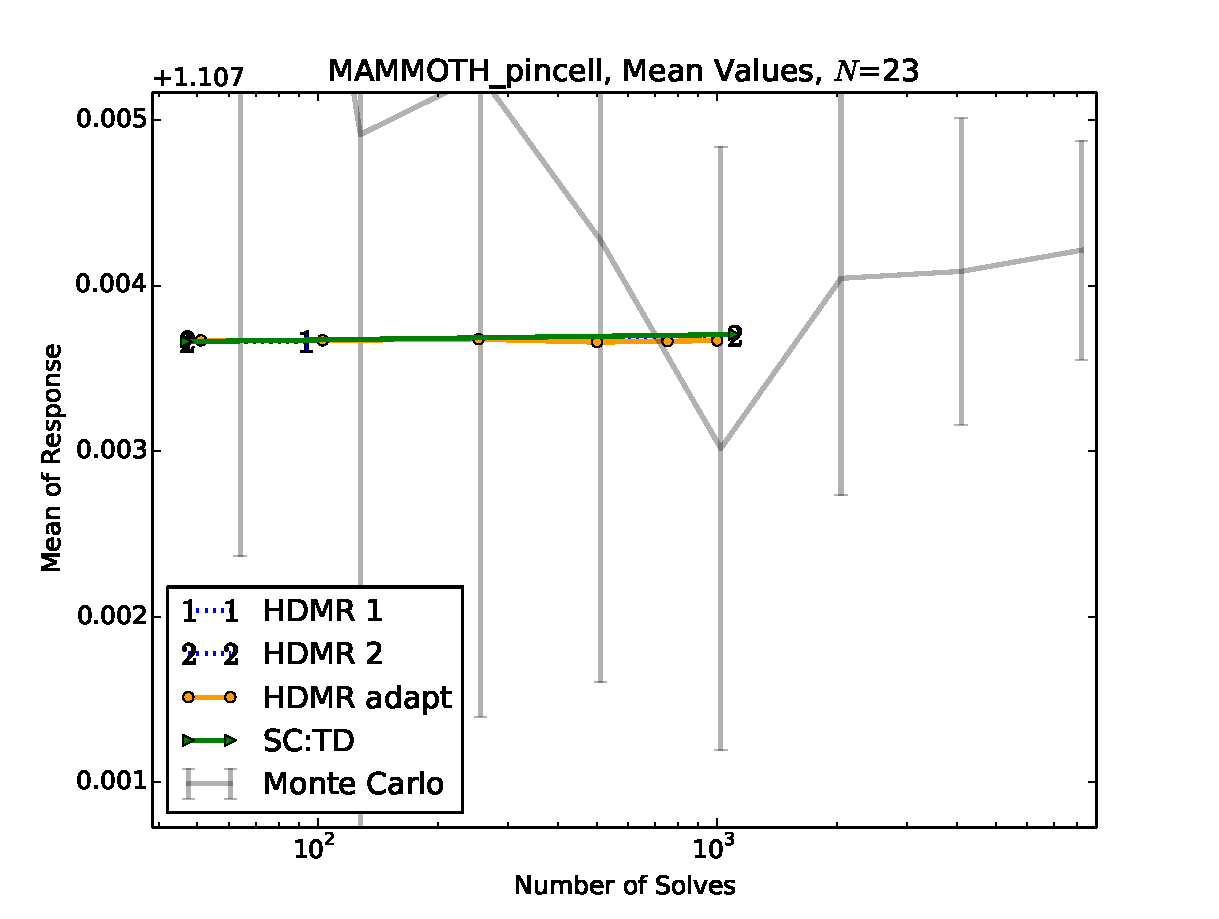
\includegraphics[width=0.7\linewidth]{mammoth/MAMMOTH_pincell_mean_zoom}
  \caption{MAMMOTH Pin Cell, Mean Values (Zoomed)}
  \label{fig:mammoth mean zoom}
\end{figure}
\begin{figure}[htb]
  \centering
  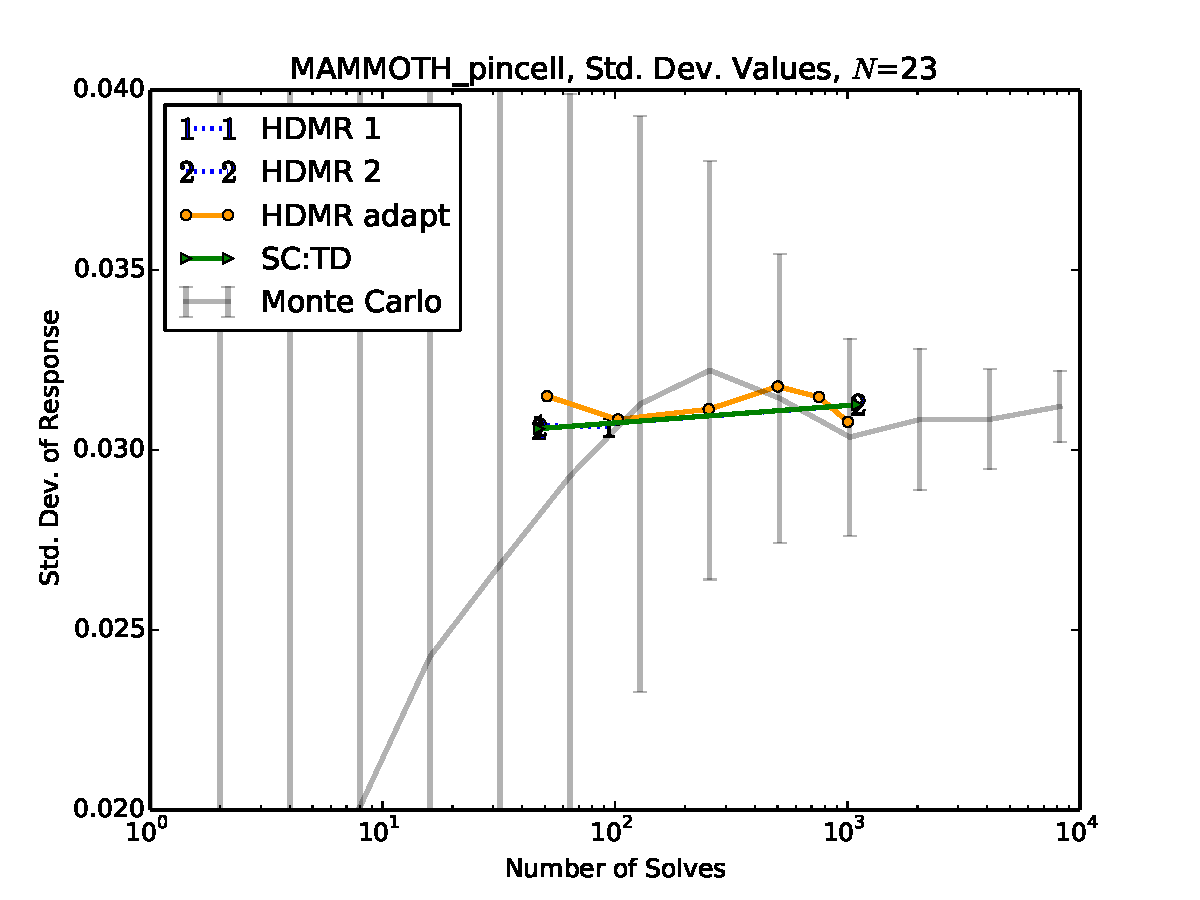
\includegraphics[width=0.7\linewidth]{mammoth/MAMMOTH_pincell_var_vals}
  \caption{MAMMOTH Pin Cell, Variance Values}
  \label{fig:mammoth var}
\end{figure}
\begin{figure}[htb]
  \centering
  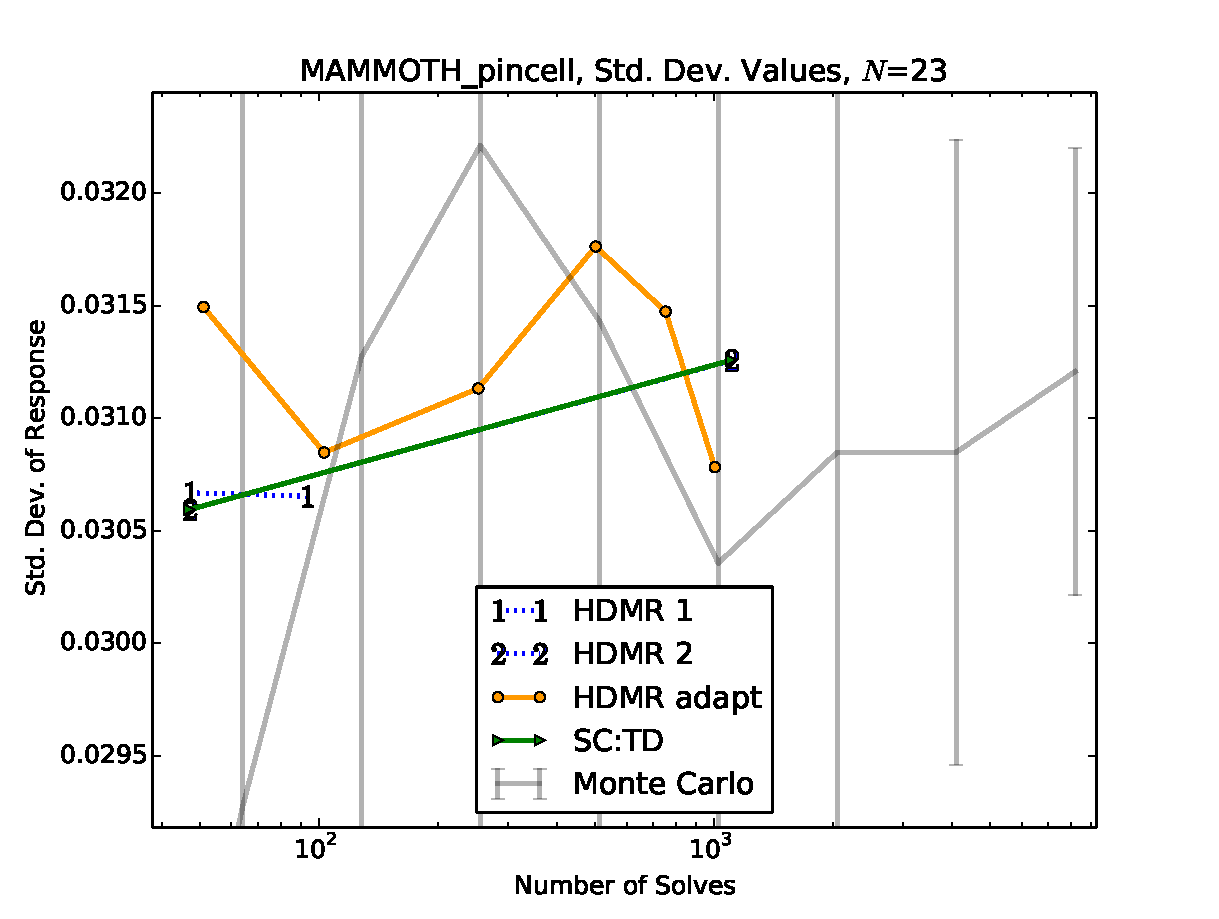
\includegraphics[width=0.7\linewidth]{mammoth/MAMMOTH_pincell_var_zoom}
  \caption{MAMMOTH Pin Cell, Variance Values (Zoomed)}
  \label{fig:mammoth var zoom}
\end{figure}

Table \ref{tab:mammoth runs} 
summarizes the number of calculations required for each collocation method.  Entries marked with a
$\dagger$ indicate results that were not obtained because of \mammoth{} simulations that failed to converge.
Entries marked with a $*$ indicate results that were not attempted because of the number of samples required.
We note that in Table \ref{tab:mammoth runs} for first-order static HDMR method successive runs have the same
number of evaluations required despite constructing higher-order polynomials.  This is because we enforced a
floor function for quadrature, requiring a minimum number of quadrature points for a polynomial despite its
low order.  This
artificially increases the points for odd-numbered sets for this particular method, but prevents abnormally
poor integration.
\begin{table}
  \centering
  \begin{tabular}{c c|c}
    Method & Degree & Runs \\ \hline
    Total Degree & 1 & 47 \\
    Total Degree & 2 & 1105 \\
    Total Degree$^*$ & 3 & 17389 \\ \hline
    HDMR (1) & 1 & 47 \\
    HDMR (1) & 2 & 47 \\
    HDMR (1) & 3 & 93 \\
    HDMR (1) & 4 & 93 \\
    HDMR (1) & 5 & 139\\ \hline
    HDMR (2) & 1 & 47 \\
    HDMR (2) & 2 & 1105 \\
    HDMR (2)$^\dagger$ & 3 & 3221 \\
    HDMR (2)$^\dagger$ & 4 & 7361 \\
    HDMR (2)$^*$ & 5 & 13571 \\
  \end{tabular}
  \caption{Evaluations Required for 23 Input Pin Cell Model}
  \label{tab:mammoth runs}
\end{table}

We observe that for both the mean and the variance, the collocation-based methods all converge within the
estimated Monte Carlo value single-standard deviation band with only first-order results.  This suggests a
high degree of linearity in the response.  In both the mean and the standard deviation, there appears to be
some convergence towards increasing the moment magnitudes from the first-order expansions, but without a near-analytic
benchmark it is difficult to be certain if this is convergence to the true solution.  

We also observe that for the standard deviation, second-order truncated HDMR matches the Total Degree SCgPC
line almost exactly.  This is expected because the HDMR subsets are constructed using the Total Degree index
set construction method; as a result, the two have identical form for up to second-order polynomial
terms.

\section{Conclusions}
While the lack of an analytic benchmark makes it difficult to be certain how much better the collocation-based
methods are performing than traditional MC, it is clear they are no worse even with first-order
approximations.  With these first-order approximations only requiring roughly 47 evaluations
instead of ten thousand, we are prepared to conclude that all the collocation-based methods considered here
are more efficient for this response than traditional analog Monte Carlo when determining
second-order statistics.

%Run times
%
%For Picard 6 and SN (3 azimuthal, 3 polar Gauss Chebyshev):
%
%MPI 24: 11m 29.452s = 689.452 sec =  16546.848 single equivalent (0.424 efficient)
%MPI 12: 19m 41.703s = 1181.703 sec = 14180.436 single equivalent (0.495 efficient)
%MPI  6: 27m 50.373s = 1670.373 sec = 10022.238 single equivalent (0.701 efficient)
%MPI  1: 117m 0.756s = 7020.756 sec =  7020.756 single equivalent (1.000 efficient)
